\documentclass[a4paper,10pt]{article}
\usepackage{fullpage}
\usepackage{amsfonts}
\usepackage[utf8]{inputenc}
\usepackage[english]{babel}
\usepackage{amsmath}
\usepackage{indentfirst}
\usepackage{graphicx}
\usepackage{natbib}
\bibliographystyle{apalike}


\begin{document}
\begin{center}
Project report on\\
\vspace{0.5cm}
{{\Large \sc Artificial Intelligence Playing the Ricochet Robots Board Game}} \\
\vspace{0.5cm} for 02180 Introduction to Artificial Intelligence
\end{center}
\rule{\textwidth}{0.5pt}
\begin{description}
\item\begin{tabular}{rll}
    \textbf{Contributors:}  & Jannis Haberhausen  & (s186398) \\ 
                            & Jack Reinhardt      & (s186182) \\ 
                            & Kilian Speiser      & (s181993) \\ 
                            & Jacob Miller        & (s186093) \\
\end{tabular}
\end{description}
\rule{\textwidth}{1pt}

\tableofcontents
\thispagestyle{empty}
\newpage

\section{Game Background}
\textit{Ricochet Robots} is a competitive game first published in Germany in 1999. It can be played with two or more people. The objective of the game is to move robots over the board such that one of the robots reaches a designated target. All players simultaneously try to find a solution to the given search problem. In order to do that every player is allowed to move all robots. That means all players are provided with perfect information and makes the game deterministic and fully observable. 

  \subsection{Game Rules}
  \label{subsec:gameRules}
  In the original game, four different colored robots are placed on a 16 by 16 board.
  The objective of the game is to reach a target that is placed somewhere on the board each round. The targets have different colors matching the colors of the four robots.
  A red target has to be reached by the red robot, a blue target by the blue robot and so on. The challenge of the game comes from the allowed movements of the robots. All
  robots can move in four directions: up, down, left and right, however once a robot is moved it will only stop when it hits a wall or another robot. The outer edges of the
  board, the four middle squares as well as additional squares on the board are blocked on up to two sides by walls. In order to reach the target, sometimes robots of other colors
  need to be used as 'walls'.
  \begin{figure}[!htb]
  \center{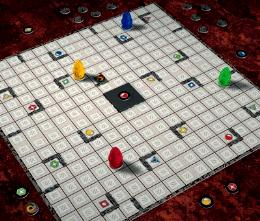
\includegraphics[width=6cm]{figures/originalgame.jpg}}
  \caption{The boardgame 'Ricochet Robots'}
  \label{fig:originalgame}
  \end{figure}

  \subsection{Changes in the Implementation}
  In the original game the board consists of four quarters printed on both sides that can be put together such that 96 unique board setups are possible. In a later version of the
  game there are eight quarters resulting in 1536 possible board configurations. For the assignment only one, randomly chosen, board configuration from the original game has been
  implemented. All game setups from the board game contain 17 targets, four in each color and one special target that has no individual color but counts as a target for every
  robot. To choose which target is the current goal in the board game one player picks and turns over a card that reveals the information to every player at the same time. With
  our implementation, only one target is drawn on the board at a time. The target is randomly placed on a square of the board that is shielded by exactly two walls, but not in one of the corners of the board (just like all the target squares in the original game).
  \par
  In order to run tests on the AI algorithms, an additional 6 by 6 board has been implemented. The game rules are exactly the same, only some squares have walls on three sides.
  The small board achieves a smaller state space and less complexity as discussed in Section \ref{sec:stateSpace}.
  \begin{figure}[!htb]
  \center{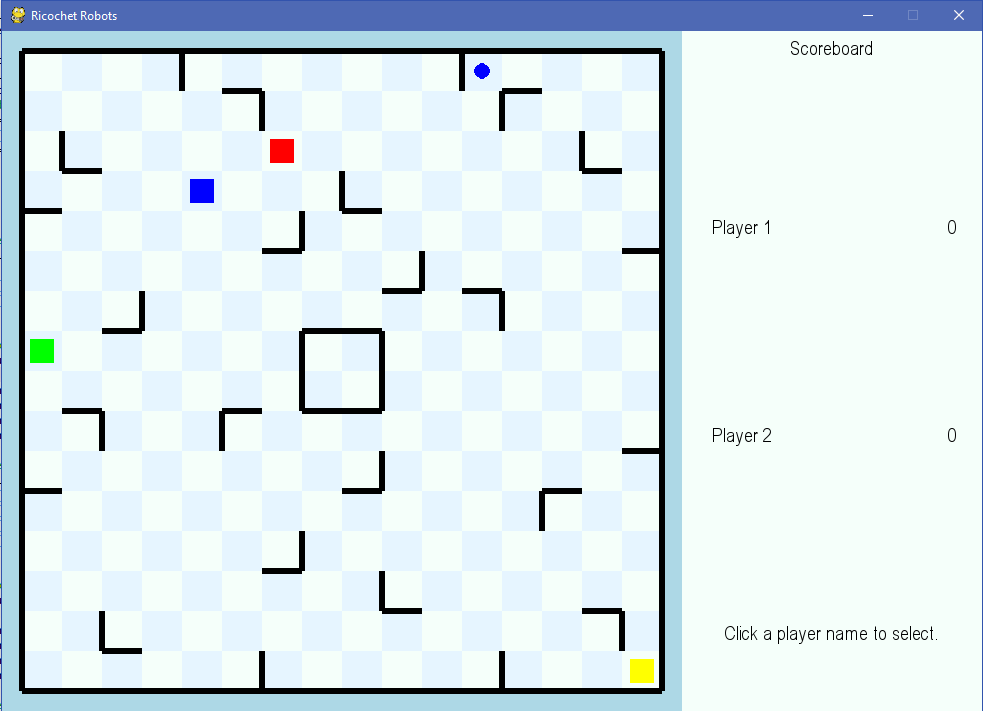
\includegraphics[width=10cm]{figures/boardimplementation.png}}
  \caption{The implementation of 'Ricochet Robots'}
  \label{fig:implementation}
  \end{figure}

  \subsection{Applicable AIs}
  As \textit{Ricochet Robots} is not adversarial (in fact for the AI implementation it is essentially a one player game with the challenge to perform better than a previous player) the Minimax-Algrothim and Monte-Carlo-Tree-Search are not applicable. \\
  Instead graph and tree searches with Depth-First-Search (dfs), Breath-First-Search (bfs) and A* were implemented. Different techniques were explored to optimize the performance of the search algorithms which are presented in section \ref{sec:searchAlgorithms}. In section \ref{sec:futureWork} ideas for more advanced AIs that try to mimic human reasoning and intuition are presented.

\section{Game Representation}
\label{sec:gameRep}
The representation of the game state only includes the locations of the game pieces - the robots - and the location of the target. The walls on the board are static,
so these are not included in the game state. More specifically, the state is represented by a tuple of robots, and the target. The possible moves, dictated by Section
\ref{subsec:gameRules}, can be retrieved from the tuple in conjunction with the static game board. There is perfect observability in the game, so there is no need to represent
the game state as a belief state. The state is simple to represent, which makes the AI algorithms run more efficiently and accurately.

\section{State Space and Complexity}
\label{sec:stateSpace}
The state space and branching factor of Ricochet Robots is large, making the task of reaching the target non-trivial for both humans and AI search algorithms.
The board consists of a 16x16 grid with walls placed in predetermined positions.  With four robots that can be moved anywhere on the board (other
than on top of another robot or the four middle squares), this leaves a total of $(16*16-4)(16*16-5)(16*16-6)(16*16-7) = 3,937,437,000$ board configurations for a single wall setup and
target placement.  Depending on the board setup, some states may not be reachable, but the state space still remains large. Each robot can move in any of the
four directions on the board until it reaches a wall or another robot in its path.  Assuming that each robot has an obstruction in one of the four directions
decreases the possible moves for each robot to three, giving the search algorithm a branching factor of $4*3 = 12$.  This assumption will be true in most cases since
the robot must be stopped by an obstruction before moving in a different direction. \\

The large state space and branching factor makes the problem of reaching the goal state difficult for traditional AI search algorithms with limited memory and time.
In order to simplify the game and drastically reduce the size of the state space and the branching factor, we implemented Ricochet Robots in a way that allows the
user to choose the size of the board (16x16 or 6x6) as well as the number of robots. In general, the size of the state space can be approximated by $(w*h)^n$ and
the branching factor can be approximated by $n*3$, where w is the board width, h is the board height and n is the number of robots.  This reduced implementation of
Ricochet Robots allowed us to play and test our AI algorithms without surpassing our memory and time limitations.


\section{Search Algorithms and Results}
\label{sec:searchAlgorithms}
  \subsection{Recursive Depth-Limited Search} \label{recursiveDFS}
  Given the large branching factor of Ricochet Robots, a depth-limited search gives the AI player a higher potential to find solutions to the more difficult board
  configurations.  Some experimentation is necessary to find the optimal limit to the depth, but when the AI player is attempting to find a better solution than
  its human competitor, the limit could simply be set to one less than the human move count.  \\

  Specific design choices were made in order to optimize the depth-limited search for Ricochet Robots.  The depth-limited search was implemented recursively and
  as a tree search rather than a graph search.  Not keeping track of past states gives the algorithm much less overhead and allows it to expand nodes more quickly,
  increasing the success rate.  The algorithm will start in the initial state by looping through each possible move for each robot and continue traversing the tree
  recursively until it either reaches a solution or it reaches the specified depth limit.  Once it reaches the depth limit, it will return to the previous level of
  recursion to search the next branch at that depth. For example, if the depth limit is set to ten, the algorithm will traverse down one path, with the direction being
  randomly determined at each move, until it is ten moves away from the initial state, at which point it will return to the depth of nine to test all other moves on
  that branch and so on. \\

  One negative aspect of the depth-limited AI player is that it usually does not find an optimal solution.  Most solutions contain extraneous moves that do nothing
  towards reaching the goal state.  In order to alleviate this issue, two aspects were added to the algorithm.  First, when checking if a move is possible, the
  algorithm also checks if the move is the opposite of the previous move (i.e if the red robot just moved North, do not allow it to move South).  This cuts off an
  entire repeated branch of the search tree, giving the algorithm more time to search new branches.  Second, once the algorithm finds a solution, it will optimize it
  by removing non-essential moves.  It does this by iteratively deleting moves from the end and testing if the goal state is still reached. \\

  \begin{figure}[h!]
    \centering
   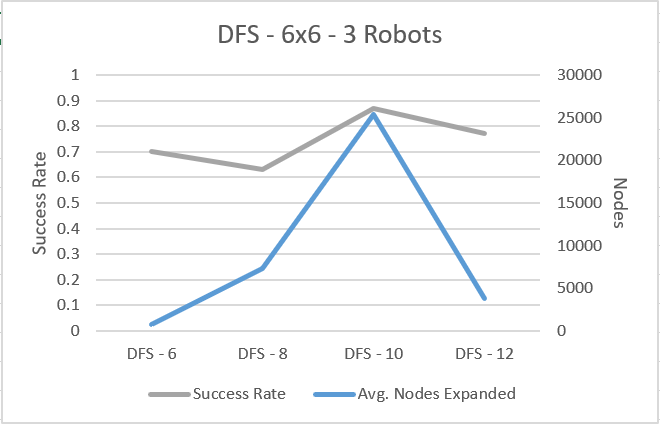
\includegraphics[width=0.45\linewidth]{figures/img1.PNG}
    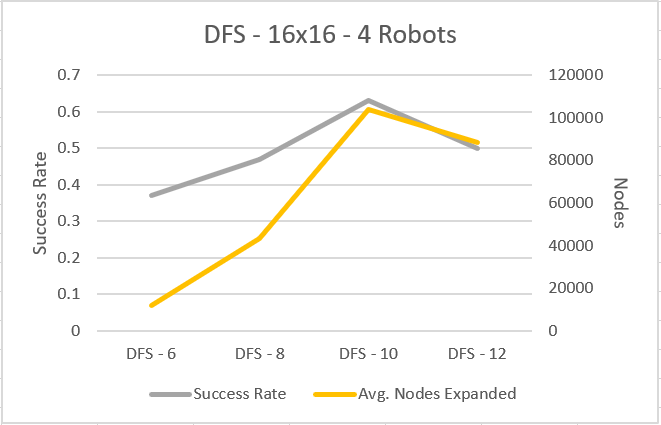
\includegraphics[width=0.45\linewidth]{figures/img2.PNG}
    \caption{Depth-limited Search Testing Results}
    \label{fig:DFS_chart}
  \end{figure}

  Figure \ref{fig:DFS_chart} shows the testing results for the depth-limited search with different maximum depth limits.  Each algorithm was tested on 30 iterations
  of Ricochet Robots, starting with a random board setup and continuing the next round where the previous round left each of the robots.  Each iteration placed the
  target randomly, meaning that some configurations may be more difficult to find a solution or the optimal solution may be at a larger depth.  The AI player was
  given sixty seconds to find a solution. \\

  For both the simplified implementation (6x6 board and three robots) and the full implementation (16x16 board and four robots), a depth limit of ten was able to
  find a solution most frequently.  Depth limits of six and eight performed considerably worse than that of ten for both tests, implying that many of the solutions were
  past these depth limits.  The AI player with a depth limit of twelve performed poorly on the simplified implementation, but only marginally worse than that of ten in
  the full implementation.  This is likely because the algorithm wastes time searching deep into branches of the search tree when the solutions to the simplified game
  are closer to the initial state.  Overall, the depth-limited AI player would be an adequate match for a human player in both the full and simplified versions of
  Ricochet Robots.\\

  \subsection{Informed Breadth-First Search}
  \begin{figure}
  	\centering

  	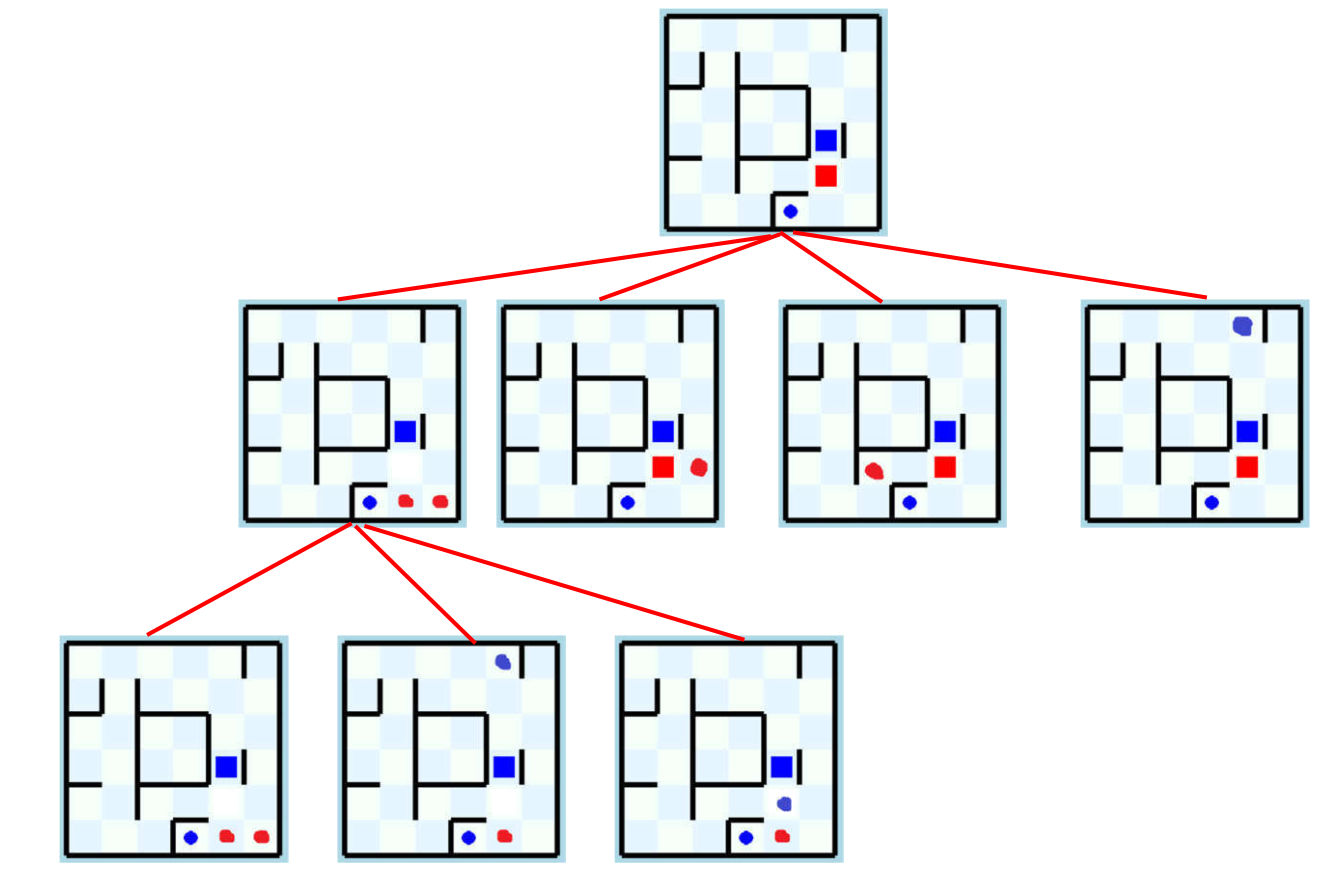
\includegraphics[scale=0.50]{figures/bfs_tree.PNG}
  	\caption{Breadth First Search Search Tree built}
  	\label{fig:bfs_tree}
  \end{figure}
  Another way to find a solution for searching problems is a breadth-first approach. This search expands all nodes on the current level before it explores the nodes on the lower level. Therefore, it always finds the optimal solution. However, considering the game state of Ricochet Robots, the search tree expands quickly, and the algorithm becomes slow. Figure \ref{fig:bfs_tree} shows how the algorithm works. Given a certain game state, the search moves one robot in each direction. If it does not reach the target and the new game state is not already saved on the frontier or expanded-nodes queue, then it is added to the frontier. The algorithm does that for all possible directions and robots before it expands the next game state from the frontier. If the target is reached, the algorithm returns the node of the goal state. The moves to reach the goal can be reconstructed by iterating through all the father nodes as the node class contains the move of how a certain game state is reached. The implementation does follow the code in \cite{Textbook} with one difference. The code in \cite{Textbook} chooses the node from the frontier and compares if it equals the goal state. Therefore, it may add a game state already has reached the square with the target. Considering the high branching, the algorithm must explore many nodes before it finds the solution. This AI compares it directly after moving the robot to preclude that the search explores additional nodes even though the robot already reached the target.\\
	  \begin{figure}
	  	\centering
	  	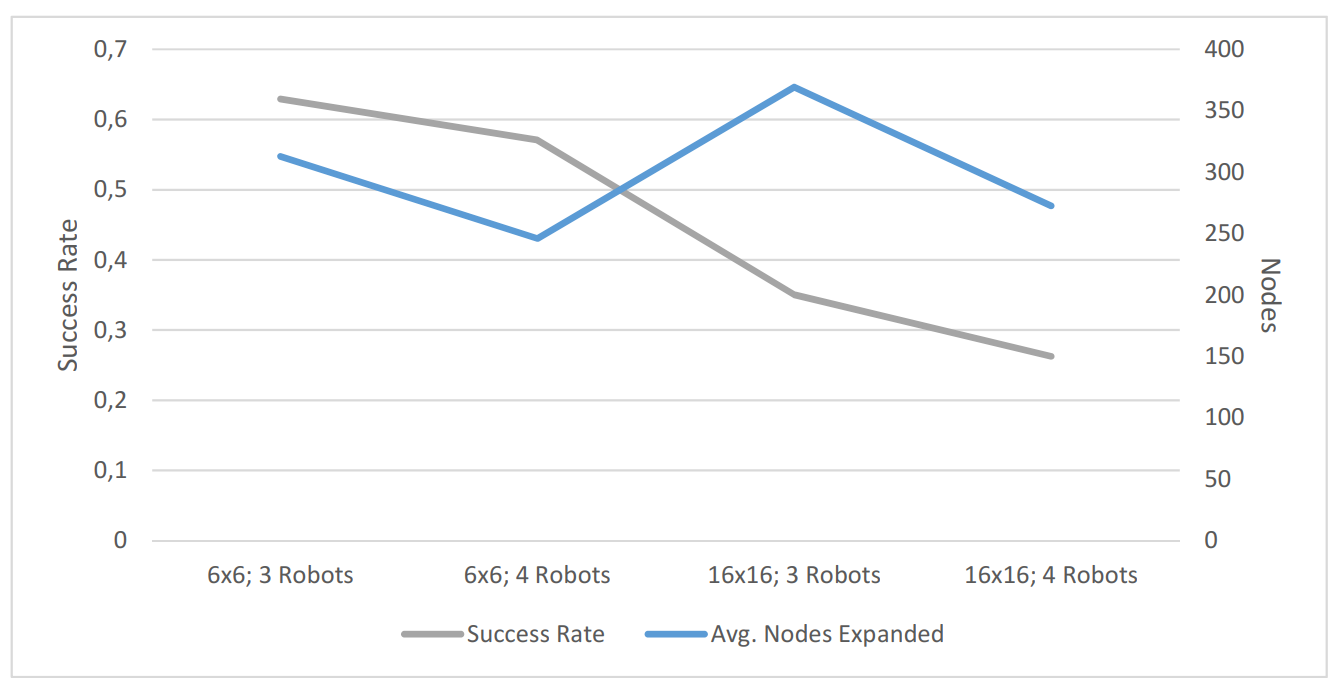
\includegraphics[scale=0.47]{figures/Bfs_test_results.PNG}
	  	\caption{Breadth First Search testing results.}
	  	\label{fig:bfs_test}
	  \end{figure}
  The algorithm is tested on two different board sizes and both, three and four robots. Figure \ref{fig:bfs_test} shows the results. While the amount of expanded nodes depends on the number of robots, the success rate depends on the board size and the numbers of robots. Compared to the depth-first search, the breadth-first search finds a solution less frequently. One reason for that is that it follows branches without utility to reach the target. Therefore, the following section integrates a heuristic function.

  \subsection{A* Search}
  Two heuristic functions were tested with the A* graph search for their ability to quickly reach the target in Ricochet Robot.
  \begin{enumerate}
    \item Manhattan Distance - let h be equal to the one-norm of the target's location on the board and the location of the robot of corresponding color. \\
    $h = |robots.x - target.x| + |robots.y - target.y|$
    \item Row/Column - for each robot accumulate h according to the following:
    \begin{itemize}
      \item[--] if the robot color matches the target color, then h += 0 if the robot is in the same row or column as the target and h += 1 otherwise
      \item[--] else, h += 0 if the robot is in an adjacent row or column to the target and h += 1 otherwise
    \end{itemize}
  \end{enumerate}
  Neither heuristic function is consistent and therefore this algorithm does not guarantee an optimal solution.  While a breadth-first search is optimal,
  it is increasingly slow at each depth level due to the large branching factor.  The A* search would prioritize certain nodes to expand based on the heuristics
  defined above, hopefully allowing it to reach the target more quickly. \\
  \begin{figure}[h!]
    \centering
    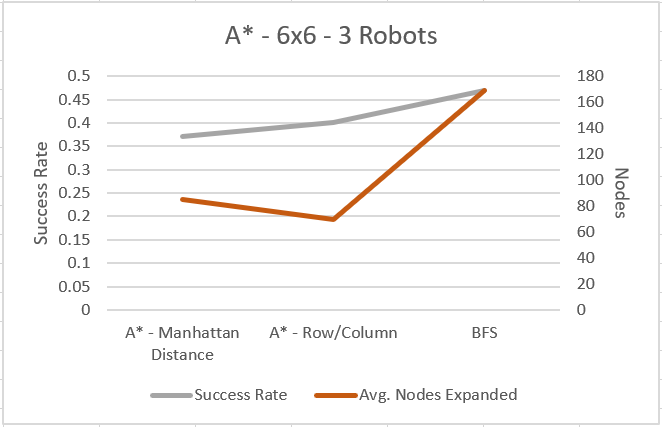
\includegraphics[width=0.45\linewidth]{figures/img3.PNG}
    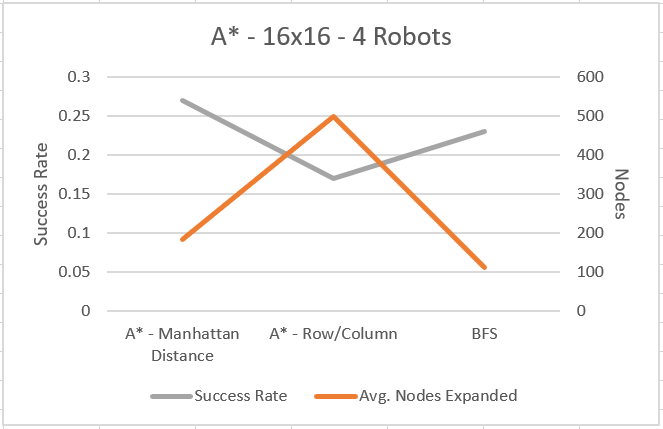
\includegraphics[width=0.45\linewidth]{figures/img4.PNG}
    \caption{A* Testing Results}
    \label{fig:A*_chart}
  \end{figure}
  Figure \ref{fig:A*_chart} shows the testing results for the A* AI player given the two heuristic functions described above as well as a breadth-first search as a
  baseline (setting h = 0).  Paralleling the tests done with the recursive depth-limited search algorithm, each AI player was tested on 30 random iterations of Ricochet
  Robots with a time limit of sixty seconds. \\
  While BFS performed the best in the simplified implementation, it was beat out by the A* - Manhattan Distance in the full implementation.  BFS will perform best when
  the goal state is at a shallow depth because it is optimal and therefore will never skip over a solution close to the initial state.  This behavior explains BFS's
  success in the simplified game.  Unfortunately, BFS will not be able to search deeper states in the search tree before it runs out of time.  The Manhattan distance
  heuristic is not optimal, which may cause it to miss some shallower solutions that BFS would find, but in the full game the heuristic seems to have helped guide the AI
  player towards a solution quicker than BFS.  The row/column heuristic performed worst in both games and does not seem to be a viable algorithm for Ricochet Robots.
  Due to the higher memory usage and slower run-time per iteration associated with the A* AI player, it cannot search nearly as many states as the recursive depth-limited
  AI player, and therefore had far lower success rates than that of the recursive depth-limited AI player.

\section{Future Work}
\label{sec:futureWork}

  \subsection{Game Improvements}
  Implementing either a randomazied boardsetup (random placement of walls) or different quaters that can be combined to different setups, similar to the original boardgame would improve the variety of the game. Additionally, using more space efficient data structures would speed up the processes of the game. For example, we could use bits to encode the game board instead of objects. This would greatly reduce space and boost the speed of all search algorithms.

  \subsection{Search Algorithm combined with human intuition}
  In figure \ref{fig:pseudo} the ideas for an advanced AI that tries to mimic human reasoning and intuition are layed out. 
  \begin{figure}[!htb]
  \center{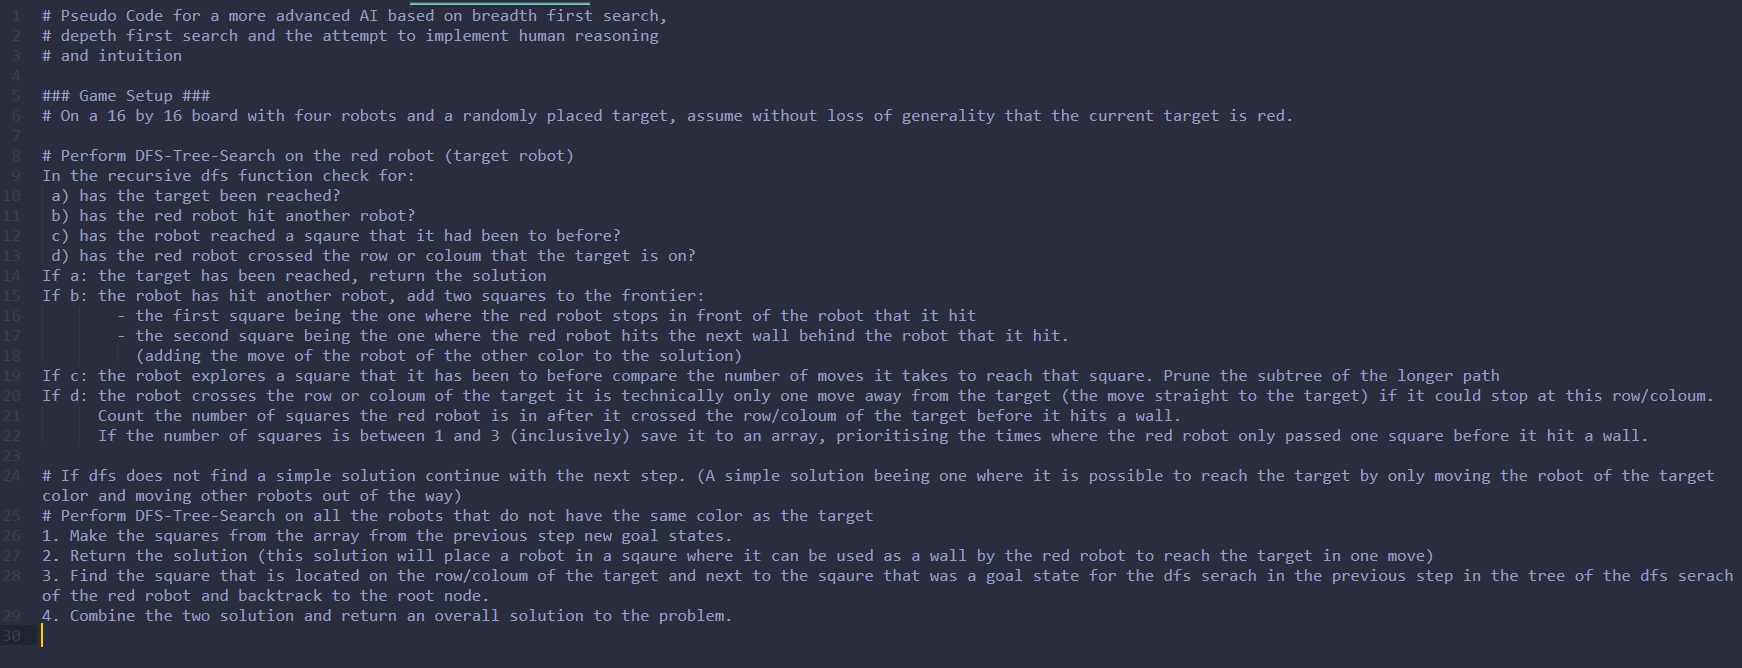
\includegraphics[width=\textwidth]{figures/pseudocode.png}}
  \caption{The 'pseudo code' for a more advanced AI}
  \label{fig:pseudo}
  \end{figure}

\section{Conclusion}
Three AI algorithms, depth-limited search, breadth-first search, and A* search, were tested for their ability to consistently reach the target in Ricochet Robots. After numerous tests of each algorithm, the depth-limited search is the most worthy human competitor due to its ability to quickly search through many states while optimizing the solution once a path to the target is found.
While breadth-first search is optimal, giving it an advantage in some instances, the breadth-first and A* graph search algorithms often times could not reach the depth necessary to find a solution.
The success of each algorithm is of course dependent on the hardware of the computer since the AI player will only have one minute to find a solution. A custom search
algorithm was devised but not implemented and could be explored for future work.

\bibliography{bib/bib}

\end{document}
